% =====================================================
% 第2章:CMOS構造進化と三次元化の展開(💯最終版)
% =====================================================
\chapter{CMOS構造進化と三次元化の展開}

本章では、プレーナーMOS構造の電界制御限界を出発点として、  
FinFET、GAA、CFETへと進化したCMOS三次元構造の系譜を整理する。  
構造スケーリングは、単なる寸法縮小ではなく、「電界制御を立体化する」設計転換である。

% -----------------------------------------------------
\section{プレーナーMOS構造の限界}
プレーナーMOSFETでは、チャネル長の短縮に伴いドレイン電界がチャネル領域に侵入し、  
短チャネル効果(SCE)およびドレイン誘起バリア低下(DIBL)が顕著となる。  
これによりしきい値電圧の低下とリーク電流増大が発生し、従来のDennardスケーリングは成立しなくなった。

130\,nm世代以降ではゲート酸化膜厚が数\si{\nano\meter}となり、  
トンネル電流によるリークが支配的となる。  
この限界を克服するため、ゲートを立体的に包み込むFinFET構造が登場した。

\begin{figure}[t]
  \centering
  % figs/fig_planar_sce.tex
% プレーナーMOSのSCE模式図(モノクロ・1カラム適合)

\tikzset{
  gate/.style   ={pattern=north east lines, pattern color=black, draw=black},
  oxide/.style  ={fill=black!7, draw=black},
  si/.style     ={fill=white, draw=black},
  sd/.style     ={fill=black!25, draw=black},
  field/.style  ={->, line width=0.3pt},
  label/.style  ={font=\footnotesize}
}
\begin{tikzpicture}[scale=0.95]
  % Substrate
  \draw[fill=black!10,draw=black] (-0.4,0) rectangle (4.4,-0.5);
  \node[label] at (2.0,-0.7) {Si Substrate};

  % Oxide + channel slab
  \draw[oxide] (0,0) rectangle (4,1.2);   % STI/BOX-ish region
  \draw[si]    (0.4,0.2) rectangle (3.6,0.6); % channel slab

  % Gate oxide + gate
  \draw[oxide, line width=0.4pt] (0.4,0.6) rectangle (3.6,0.7);
  \draw[gate]  (0.8,0.7) rectangle (3.2,1.1);
  \node[label] at (2.0,1.25) {Gate};

  % Source / Drain
  \draw[sd] (0.0,0.2) rectangle (0.4,0.9);
  \draw[sd] (3.6,0.2) rectangle (4.0,0.9);
  \node[label] at (0.2,1.05) {S};
  \node[label] at (3.8,1.05) {D};

  % Short-channel effect: field lines from D into channel
  \foreach \y in {0.25,0.35,0.45,0.55} {
    \draw[field] (3.8,\y) .. controls (3.1,\y+0.15) and (2.6,\y+0.05) .. (2.2,\y+0.02);
  }

  % Labels
  \node[label,align=left] at (3.2,0.2) {Drain電界の侵入\\(DIBL, SCE)};
  \node[label] at (2.0,0.0) {};
\end{tikzpicture}

  \caption{プレーナーMOSFET構造と短チャネル効果の模式図。}
\end{figure}

% -----------------------------------------------------
\section{FinFET構造:三面ゲートによる電界制御の強化}
FinFETは、立体的に形成されたシリコンフィンをゲートが三方向から包み込む「Tri-Gate」構造を有する。  
この三面ゲートにより、チャネル電位分布が体積的に制御され、SCEとDIBLが大幅に緩和される。  

Finの高さ$H$、幅$W$、本数$n$に対して有効チャネル幅は次式で表される:
\[
W_{\mathrm{eff}} = n(2H + W)
\]
側面電流が支配的であり、高Fin化により$I_{\mathrm{ON}}$を増大できる一方、加工ばらつき(LER)や段差被覆性が信頼性を制限する。  
FinFETは「平面電界制御」から「体積電位制御」への転換点である。

\begin{figure}[t]
  \centering

  % ---------- TikZ Styles ----------
  \tikzset{
    gate/.style   ={pattern=north east lines, pattern color=black, draw=black, line width=0.3pt},
    oxide/.style  ={fill=black!8, draw=black, line width=0.3pt},
    si/.style     ={fill=white, draw=black, line width=0.4pt},
    sd/.style     ={fill=black!25, draw=black, line width=0.3pt},
    substrate/.style={fill=black!15, draw=black, line width=0.3pt},
    label/.style  ={font=\footnotesize},
    dim/.style    ={-{Latex[length=2mm]}, line width=0.3pt}
  }

  % ---------- Drawing ----------
  \begin{tikzpicture}[scale=1.05]

    % Substrate
    \draw[substrate] (-0.5,0) rectangle (4.5,-0.5);
    \node[label] at (2.0,-0.8) {Substrate};

    % STI / isolation background
    \draw[oxide] (0,0) rectangle (4,1.5);

    % Fin (Si)
    \draw[si] (1.75,0) rectangle (2.25,1.2);

    % Gate oxide (thin)
    \draw[oxide] (1.65,0) rectangle (2.35,1.22);

    % Gate electrode (3 sides)
    \draw[gate] (1.35,0.2) rectangle (2.65,1.15);

    % Source / Drain
    \draw[sd] (0.25,0.2) rectangle (1.35,1.15);
    \draw[sd] (2.65,0.2) rectangle (3.75,1.15);

    % Labels (non-overlapping)
    \node[label] at (0.8,1.35) {Source (S)};
    \node[label] at (3.2,1.35) {Drain (D)};
    \node[label,align=center] at (2.0,1.4) {Gate};
    \node[label] at (2.0,0.6) {Fin (Si)};

    % Dimension arrows
    \draw[dim] (1.75,0.0) -- ++(0,1.2) node[midway,left=2pt,label] {$H$};
    \draw[dim] (1.75,1.25) -- ++(0.5,0) node[midway,above=2pt,label] {$W$};

  \end{tikzpicture}

  % ---------- Caption ----------
  \caption{FinFETの断面模式図(高精細版)。ゲート電極は三面を包囲し、Finの幾何パラメータ $H,\,W$ は有効チャネル幅 $W_{\mathrm{eff}} = n(2H + W)$ に寄与する。}
  \label{fig:finfet_detail}
\end{figure}


% -----------------------------------------------------
\section{GAA構造:全包囲ゲートへの発展}
GAA(Gate-All-Around)は、チャネルを上下左右すべての面からゲートで包み込む構造であり、  
FinFETの静電制御性を極限まで高めたデバイスである。  
複数のナノシートを積層して構成され、上下両面の電流経路が追加されるため、  
同一フットプリントでより高い駆動能力を実現する。

\[
W_{\mathrm{eff}} = 2n(H + W)
\]
ここで$n$はシート層数である。  
Selective Epitaxial Growth(SEG)とAtomic Layer Deposition(ALD)による膜厚制御が鍵であり、  
GAAは「完全電界包囲デバイス」として5\,nm以降の主流技術となった。

% =====================================================
% Fig. 6 : GAA(Gate-All-Around)ナノシート構造 断面図
% =====================================================
\begin{figure}[t]
  \centering
  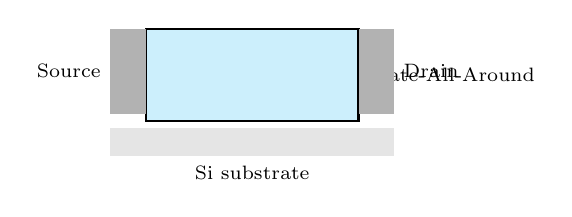
\begin{tikzpicture}[scale=0.9, every node/.style={font=\scriptsize}]
    % substrate
    \fill[gray!20] (0,0) rectangle (4,0.4);
    \node[below] at (2,0) {Si substrate};

    % nanosheets (3層)
    \foreach \y in {0.6,1.0,1.4} {
      \fill[orange!30] (0.8,\y) rectangle (3.2,\y+0.2);
      \draw[black!50] (0.8,\y) rectangle (3.2,\y+0.2);
    }

    % gate stack
    \draw[thick,fill=cyan!20] (0.5,0.5) rectangle (3.5,1.8);
    \node[right] at (3.55,1.15) {Gate-All-Around};

    % source/drain
    \fill[gray!60] (0,0.6) rectangle (0.5,1.8);
    \fill[gray!60] (3.5,0.6) rectangle (4.0,1.8);
    \node[left] at (0,1.2) {Source};
    \node[right] at (4,1.2) {Drain};
  \end{tikzpicture}

  \caption{GAAナノシート構造の模式断面図(S/D領域とゲート包囲面を示す)\\
  \footnotesize Schematic cross-section of GAA nanosheet structure showing gate wrapping around multiple stacked channels.}
  \label{fig:gaa_cross}
\end{figure}


% -----------------------------------------------------
\section{CFET構造:垂直積層による空間効率化}
CFET(Complementary FET)は、n型とp型のFETを垂直方向に積層した三次元構造である。  
GAA技術を前提に、Backside Power Rail(BPR)と統合することで、  
セル面積を大幅に削減し、信号配線と電源配線を分離できる。  

上下FET間の熱干渉や電気的アイソレーションの確保が設計上の要となる。  
熱対称性(thermal symmetry)を維持しつつ、<400°C低温プロセスによる層間分離を実現することが  
次世代1\,nmノードでの信頼性を左右する。

% =====================================================
% Fig. 7 : CFET(Complementary FET)垂直積層構造 断面図
% =====================================================
\begin{figure}[t]
  \centering
  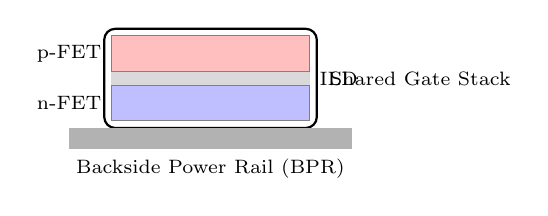
\begin{tikzpicture}[scale=0.9, every node/.style={font=\scriptsize}]
    % bottom n-FET
    \fill[blue!25] (0.6,0.4) rectangle (3.4,0.9);
    \draw[black!50] (0.6,0.4) rectangle (3.4,0.9);
    \node[left] at (0.6,0.65) {n-FET};

    % isolation (ILD)
    \fill[gray!30] (0.6,0.9) rectangle (3.4,1.1);
    \node[right] at (3.4,1.0) {ILD};

    % top p-FET
    \fill[red!25] (0.6,1.1) rectangle (3.4,1.6);
    \draw[black!50] (0.6,1.1) rectangle (3.4,1.6);
    \node[left] at (0.6,1.35) {p-FET};

    % gate stack
    \draw[thick,rounded corners] (0.5,0.3) rectangle (3.5,1.7);
    \node[right] at (3.55,1.0) {Shared Gate Stack};

    % backside power rail (BPR)
    \fill[gray!60] (0,0) rectangle (4,0.3);
    \node[below] at (2,0) {Backside Power Rail (BPR)};
  \end{tikzpicture}

  \caption{CFET構造の垂直積層模式図(n/pスタックおよびBPRを示す)\\
  \footnotesize Schematic vertical stack of CFET showing n/p layers and backside power rail.}
  \label{fig:cfet_cross}
\end{figure}


% -----------------------------------------------------
\section{構造比較:FinFET-GAA-CFETの連続性}
FinFET、GAA、CFETの三構造は、電界制御の立体化と配線分離効率の進化を示す連続系列である。  
FinFETは三面制御、GAAは全包囲制御、CFETはさらに上下分離による電源・信号統合を達成する。  

この流れは「電界制御 → 空間効率 → 電源分離」という  
スケーリング軸の深化を象徴しており、構造そのものが  
デバイス性能と信頼性を同時に規定する時代への転換点である。

\begin{figure}[t]
  \centering
  \begin{figure}[t]
  \centering
  \tikzset{
    gate/.style   ={pattern=north east lines, pattern color=black, draw=black},
    oxide/.style  ={fill=black!5, draw=black},
    si/.style     ={fill=white, draw=black},
    sd/.style     ={fill=black!25, draw=black},
    metal/.style  ={fill=black!40, draw=black},
    label/.style  ={font=\footnotesize},
    dim/.style    ={-{Latex[length=2mm]}, line width=0.3pt}
  }

  %=== 1) FinFET ===
  \begin{tikzpicture}[scale=0.9]
    \node[label, anchor=west] at (-0.2,3.4) {\textbf{(a) FinFET}};
    % substrate & STI
    \draw[fill=black!10, draw=black] (-0.5,0) rectangle (4.5,-0.6);
    \node[label] at (2,-0.8) {Substrate};
    \draw[oxide] (0,0) rectangle (4,1.6); % BOX/STI領域
    % fin
    \draw[si] (1.7,0) rectangle (2.3,1.4);
    % gate oxide wrapper (薄層表示)
    \draw[oxide, line width=0.4pt] (1.6,-0.02) rectangle (2.4,1.42);
    % gate metal (3面ラップ)
    \draw[gate] (1.35,0.2) rectangle (2.65,1.25);
    % source/drain
    \draw[sd] (0.25,0.2) rectangle (1.35,1.25);
    \draw[sd] (2.65,0.2) rectangle (3.75,1.25);
    \node[label] at (0.8,1.45) {S};
    \node[label] at (3.2,1.45) {D};
    \node[label] at (2.0,1.55) {Fin (Si)};
    \node[label] at (2.0,0.95) {Gate};
    % dimensions (H, W)
    \draw[dim] (2.3,0.1) -- ++(0.6,0) node[right,label] {$H$};
    \draw[dim] (1.7,0.05) -- ++(-0.6,0) node[left,label] {$H$};
    \draw[dim] (1.7,1.4) -- ++(0.6,0) node[right,label] {$W$};
  \end{tikzpicture}

  \vspace{1.2ex}

  %=== 2) GAA (Nanosheet) ===
  \begin{tikzpicture}[scale=0.9]
    \node[label, anchor=west] at (-0.2,3.4) {\textbf{(b) GAA (Nanosheet)}};
    \draw[fill=black!10, draw=black] (-0.5,0) rectangle (4.5,-0.6);
    \node[label] at (2,-0.8) {Substrate};
    \draw[oxide] (0,0) rectangle (4,1.9);
    % three sheets with gate-all-around
    \foreach \y in {0.4,0.95,1.5}{
      \draw[oxide] (1.1,\y-0.22) rectangle (2.9,\y+0.22); % spacer
      \draw[si] (1.2,\y-0.12) rectangle (2.8,\y+0.12);    % sheet
      \draw[gate] (1.0,\y-0.34) rectangle (3.0,\y+0.34);  % 4面ゲート
    }
    % S/D
    \draw[sd] (0.25,0.25) rectangle (1.0,1.65);
    \draw[sd] (3.0,0.25) rectangle (3.75,1.65);
    \node[label] at (0.7,1.85) {S};
    \node[label] at (3.3,1.85) {D};
    \node[label] at (2.0,1.95) {Gate-All-Around};
    % dims for one sheet
    \draw[-{Latex[length=2mm]}] (2.8,0.95) -- ++(0.5,0) node[right,label] {$W$};
    \draw[-{Latex[length=2mm]}] (2.6,0.83) -- ++(0, -0.35) node[below,label] {$H$};
  \end{tikzpicture}

  \vspace{1.2ex}

  %=== 3) CFET (n/p stacked) ===
  \begin{tikzpicture}[scale=0.9]
    \node[label, anchor=west] at (-0.2,3.6) {\textbf{(c) CFET (n/p 垂直積層)}};
    % BPR (backside rails)
    \draw[metal] (-0.5,-0.9) rectangle (1.6,-1.3);
    \draw[metal] (2.4,-0.9) rectangle (4.5,-1.3);
    \node[label] at (0.55,-1.45) {BPR-VDD};
    \node[label] at (3.45,-1.45) {BPR-VSS};

    % substrate and window
    \draw[fill=black!10, draw=black] (-0.5,0) rectangle (4.5,-0.6);
    \node[label] at (2,-0.8) {Substrate};
    \draw[oxide] (0,0) rectangle (4,2.6);

    % lower nFET (GAA)
    \foreach \y in {0.55}{
      \draw[gate] (1.0,\y-0.3) rectangle (3.0,\y+0.3);
      \draw[oxide] (1.1,\y-0.2) rectangle (2.9,\y+0.2);
      \draw[si] (1.2,\y-0.1) rectangle (2.8,\y+0.1);
    }
    \node[label] at (3.25,0.55) {\footnotesize nFET (GAA)};

    % ILD spacer
    \draw[oxide, fill=black!12] (0,1.05) rectangle (4,1.25);

    % upper pFET (GAA)
    \foreach \y in {1.8}{
      \draw[gate] (1.0,\y-0.3) rectangle (3.0,\y+0.3);
      \draw[oxide] (1.1,\y-0.2) rectangle (2.9,\y+0.2);
      \draw[si] (1.2,\y-0.1) rectangle (2.8,\y+0.1);
    }
    \node[label] at (3.25,1.8) {\footnotesize pFET (GAA)};

    % shared S/D towers
    \draw[sd] (0.3,0.25) rectangle (1.0,2.15);
    \draw[sd] (3.0,0.25) rectangle (3.7,2.15);
    \node[label] at (0.65,2.35) {S/D};
    \node[label] at (3.35,2.35) {S/D};
  \end{tikzpicture}

  \caption{構造比較(モノクロ模式図):(a) FinFET(三面ゲート),(b) GAA(ナノシート多層),(c) CFET(n/p垂直積層+BPR整合)。灰色は誘電体,斜線はゲート金属,濃灰はソース/ドレイン。}
  \label{fig:structure_compare}
\end{figure}

  \caption{FinFET, GAA, CFET構造の比較模式図。}
\end{figure}
